\section{Introduction to SCRUM}

\subsection{Intro in PM4}

\begin{concept}{SCRUM}
    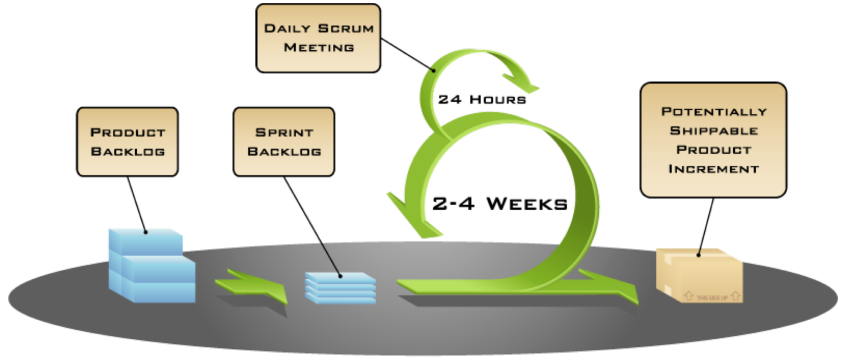
\includegraphics[width=\linewidth]{SCRUM.png}
\end{concept}

\begin{definition}{Product Backlog}
    \begin{itemize}
        \item the requirements for the product
        \item List of all desired work on the project
        \item Single source of requirements for any changes to be made to the product
        \item Prioritized by the Product Owner
    \end{itemize}
\end{definition}

\section{Einführung in Agile Software-Entwicklung}

\subsection{Traditionelle Entwicklungsmethoden}

\begin{definition}{Traditionelle Entwicklungsmethoden}\\
    Traditionelle Entwicklungsmethoden wie Wasserfall und das V-Modell sind durch einen sequenziellen Prozess gekennzeichnet:
    \begin{itemize}
        \item Vordefinierte Phasen, die nacheinander abgearbeitet werden
        \item Umfangreiche Dokumentation in jeder Phase
        \item Begrenzte Möglichkeiten für Änderungen nach Festlegung der Anforderungen
        \item Abnahme und Auslieferung erst nach vollständiger Fertigstellung
    \end{itemize}
\end{definition}

\begin{concept}{Herausforderungen in Softwareprojekten}\\
    Softwareprojekte stehen vor einzigartigen Herausforderungen:
    \begin{itemize}
        \item Komplexe, nicht-physische Produkte
        \item Anforderungen ändern sich während der Entwicklung
        \item Hohe Fehlerrate im Vergleich zu anderen Branchen
        \item Technologie entwickelt sich schneller als Methoden
        \item Weitere Faktoren: unklare Ziele, mangelhafte Führung, schlechte Kommunikation
    \end{itemize}
\end{concept}

\begin{concept}{Projektrisiko}\\
    Die Risikowahrscheinlichkeit ist in technologischen Projekten im Vergleich zu anderen Branchen überdurchschnittlich hoch.
    \begin{itemize}
        \item Studien zeigen, dass Technologieprojekte eine Erfolgsrate von nur 30-35\% haben
        \item Ähnliche Fehlerraten wären in vielen anderen Branchen nicht akzeptabel
        \item Beispiele: gescheiterte IT-Großprojekte wie "Insieme" (Schweiz), SAP-Projekte, Helvetia-IT-Projekt
    \end{itemize}
\end{concept}

\subsection{Die Entstehung von Agile}

\begin{concept}{Zentrale Fragestellung}\\
    Wie kann das Risiko in Software-Entwicklungsprojekten reduziert werden?
\end{concept}

\begin{concept}{Agile Manifesto}\\
    Im Februar 2001 trafen sich 17 Entwickler in Snowbird, Utah und formulierten das Agile Manifesto. Diese Entwickler repräsentierten verschiedene leichtgewichtige Methoden:
    \begin{itemize}
        \item Extreme Programming (XP)
        \item Scrum
        \item DSDM (Dynamic Systems Development Method)
        \item Adaptive Software Development
        \item Crystal
        \item Feature-Driven Development
        \item Pragmatic Programming
    \end{itemize}
    Sie suchten nach Alternativen zu dokumentbasierten und umfangreich geregelten Entwicklungsprozessen.
\end{concept}

\begin{definition}{Werte des Agilen Manifesto}\\
    Das Agile Manifesto definiert vier Kernwerte:
    \begin{itemize}
        \item \textbf{Individuen und Interaktion} sind wichtiger als Prozesse und Tools
        \item \textbf{Lauffähige Software} ist wichtiger als durchgängige Dokumentation
        \item \textbf{Zusammenarbeit mit dem Kunden} ist wichtiger als Vertragsverhandlungen
        \item \textbf{Auf Veränderungen reagieren} ist wichtiger als einem Plan folgen
    \end{itemize}
    "... while there is value in the items on the right, we value the items on the left more"
\end{definition}

\begin{definition}{Agile Manifesto Prinzipien}\\
    Das Agile Manifesto umfasst 12 Prinzipien:
    \begin{enumerate}
        \item \textbf{Customer Satisfaction:} Höchste Priorität hat die Zufriedenstellung des Kunden durch frühe und regelmäßige Lieferung wertvoller Software
        \item \textbf{Welcome Change:} Neue und veränderte Anforderungen sind auch spät in der Entwicklung willkommen
        \item \textbf{Deliver Frequently:} Lauffähige Software wird regelmäßig geliefert (Wochen statt Monate)
        \item \textbf{Working Together:} Fachexperten und Entwickler müssen täglich zusammenarbeiten
        \item \textbf{Motivated Team:} Projekte werden um motivierte Individuen organisiert mit der nötigen Unterstützung und Vertrauen
        \item \textbf{Face-to-Face:} Direkte Kommunikation ist die effizienteste Methode
    \end{enumerate}
\end{definition}

\begin{definition}{Agile Manifesto Prinzipien (Fortsetzung)}\\
    \begin{enumerate}
        \setcounter{enumi}{6}
        \item \textbf{Working Software:} Lauffähige Software ist das zentrale Fortschrittsmaß
        \item \textbf{Constant Pace:} Nachhaltige Entwicklung mit konstantem Arbeitstakt
        \item \textbf{Good Design:} Ständiger Fokus auf technische Exzellenz und gutes Design
        \item \textbf{Simplicity:} Die Kunst, Arbeit zu maximieren, die nicht getan werden muss
        \item \textbf{Self-Organisation:} Die besten Architekturen und Anforderungen entstehen durch selbstorganisierte Teams
        \item \textbf{Reflect \& Adjust:} Regelmäßige Reflektion und Anpassung der Arbeitsweise
    \end{enumerate}
\end{definition}

\begin{concept}{Die Variablen der Software-Entwicklung}\\
    Die vier Variablen der Software-Entwicklung:
    \begin{itemize}
        \item \textbf{Zeit:} Zeitplan für die Fertigstellung
        \item \textbf{Ressourcen:} Budget und Personal
        \item \textbf{Qualität:} Technische Funktionalität und Zuverlässigkeit
        \item \textbf{Scope:} Umfang der zu implementierenden Features
    \end{itemize}
    Externe Kräfte (Kunden, Vorgesetzte) können drei dieser Variablen definieren, das Entwicklungsteam definiert die vierte. In agilen Projekten ist typischerweise der Scope die variable Komponente.
\end{concept}

\begin{concept}{Kosten für Änderungen}\\
    Zwei unterschiedliche Sichtweisen:
    \begin{itemize}
        \item \textbf{Traditionelle Sicht:} Die Kosten für Änderungen steigen exponentiell mit dem Projektfortschritt an
        \item \textbf{Agile Sicht:} Durch moderne Praktiken (kontinuierliche Integration, automatisierte Tests, Refactoring) bleiben die Kosten für Änderungen über den Projektverlauf flacher
    \end{itemize}
\end{concept}

\begin{concept}{Grundidee hinter Agile Methoden}\\
    Der Kerngedanke ist, dass Software-Entwicklung ein empirischer Prozess ist, nicht ein definierter:
    \begin{itemize}
        \item Komplexität erfordert einen adaptiven Ansatz
        \item Regelmäßiges Inspizieren und Anpassen
        \item Lernen und Verbessern während des Projekts
        \item Risikominimierung durch frühzeitige Lieferung von Mehrwert
        \item Reaktion auf Veränderungen statt starres Befolgen eines Plans
    \end{itemize}
\end{concept}

\subsection{Die drei Gesetze der Software-Entwicklung}

\begin{concept}{Humphrey's Law}\\
    "Menschen wissen nicht, was sie wollen, bevor sie es sehen."
    
    Dieses Gesetz erklärt, warum inkrementelle Entwicklung mit regelmäßigem Feedback so wichtig ist. Es ist ein Hauptgrund, warum große Technologieunternehmen regelmäßige Releases veröffentlichen, anstatt zu versuchen, perfekte Software auf einmal zu liefern.
\end{concept}

\begin{concept}{Ziv's Law}\\
    "Softwareentwicklung ist unvorhersehbar und kann nie vollends verstanden werden."
    
    Auch bekannt als das Unsicherheitsprinzip der Softwareentwicklung. Es betont, dass komplexe Systeme inhärent schwer zu verstehen und vorherzusagen sind, was agile Praktiken zur Risikominderung notwendig macht.
\end{concept}

\begin{concept}{Conway's Law}\\
    "Software ist ein Spiegel der Firma und der Menschen, die sie entwerfen."
    
    "Organisationen, die Systeme entwerfen, sind gezwungen, Entwürfe zu erstellen, die die Kommunikationsstrukturen dieser Organisationen abbilden."
    
    Dies bedeutet, dass die Architektur eines Systems die Kommunikationsstruktur der Organisation widerspiegelt, die es erstellt hat. Die Qualität der Schnittstellen zwischen Systemkomponenten entspricht der Qualität der Kommunikation zwischen den entsprechenden Teams.
\end{concept}